\section{Auswertung}
\label{sec:Auswertung}

\subsection{Untersuchung der Filterkurve}

Für die Filterkurve wurden die folgenden \autoref{tab:tab1} Messadaten aufgenommen, dabei wurde eine 10-fache Verstärkung verwendet.

\begin{table}[H]
    \centering
    \caption{Messwerte zur Filterkurve.}
    \label{tab:tab1}
    \begin{tabular}{S S}
      \toprule
      {$f \mathbin{/} \unit{\kilo\hertz} $} & {$U \mathbin{/} \unit{\milli\volt} $}  \\
      \midrule
            10.01       &   0.5     \\
            12.95       &   0.78    \\
            16.03       &   1.11    \\
            19.03       &   2.73    \\
            20.1        &   4.4     \\
            21.0        &   8.1     \\
            22.7        &   6.9     \\
            21.1        &   8.1     \\
            30.6        &   0.84    \\
            33.0        &   0.6     \\
            36.2        &   0.51    \\
            38.3        &   0.46    \\
            40.0        &   0.4     \\
      \bottomrule
    \end{tabular}
\end{table}

Die Messwerte aus \autoref{tab:tab1} sind auch in \autoref{fig:Graph_a} dargestellt.

\begin{figure}[H]
    \centering
    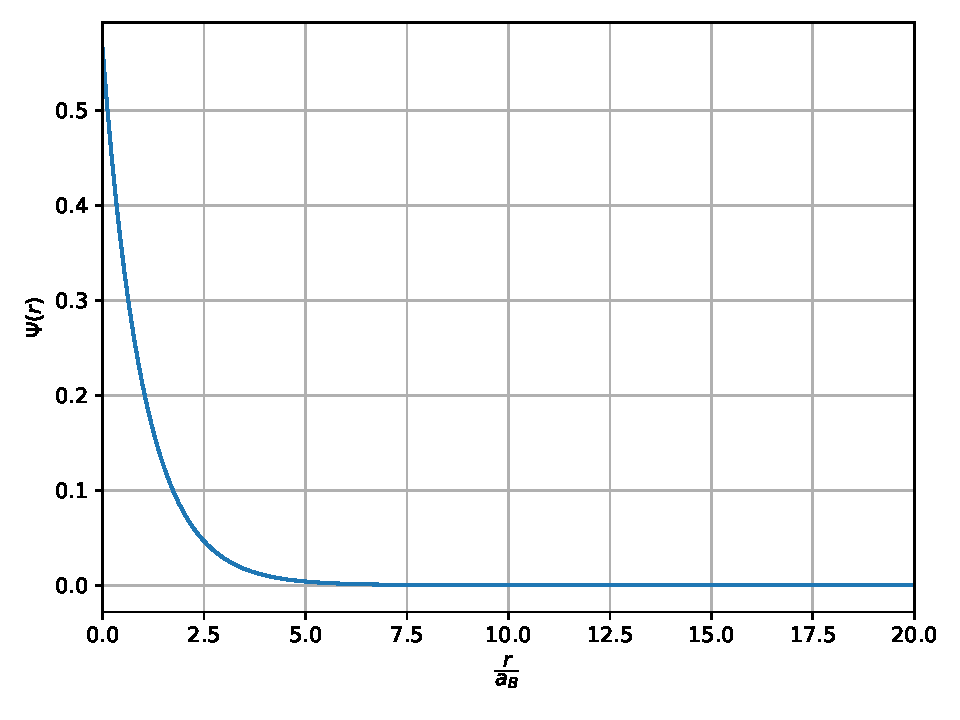
\includegraphics{build/Graph_a.pdf}
    \caption{Filterkurve der Brückenschaltung}
    \label{fig:Graph_a}
\end{figure} 

Es wurde versucht mit $ scipy$ eine Lorentzkurve der Form \eqref{eq:Lorentzkurve}, sowie eine Gaußverteilung der Form \eqref{eq:gauß} zu fitten, jedoch konnten keine Parameter, die zu den Messdaten passen gefunden werden

\begin{equation}
    f_l(v) = \frac{a}{(v^2-v_0^2)^2 + {\gamma}^2 v_0^2}
    \label{eq:Lorentzkurve}
\end{equation}

\begin{equation}
    f_g(v) = b \cdot \exp{\frac{(v-v_0)^2}{a}} \,.
    \label{eq:gauß}
\end{equation} 

Das Maximum der Spannung wird als

\begin{equation}
    U_A = 8,1 \, \unit{\volt}
\end{equation}

bei einer Frequenz von 
\begin{equation}
    v_0 = 21,05 \, \unit{\kilo\hertz}
\end{equation}
bestimmt.